
\subsection{Our voltage regulation circuit}

Our purpose was to regulate voltages and also study noise related to the circuit. If we choose a complicated circuit for voltage voltage regulation then analysis of noise will be relatively complicated. So, we used a very basic voltage regulator circuit from a zener diode. Supply was given as DC power supply with voltage $V_{s}$. This voltage is decided by the zener voltage at hand.

The noise in the circuit will be relatively higher at the zener breakdown region. As we discussed from the theoretical part, noise power will be proportional to current flowing in the zener diode (here, we are assuming that noise from other parts is almost zero). To prepare a zener diode (BZX55C5V1) to break down the region we choose 5.4V. This is calculated from 
For our purpose we utilised a general purpose zener diode with breakdown region between 4.8V to 5.4V with current of $\mu A$ order. We first did the Current and voltage characteristics of zener diodes. The useful information we got from there is source voltages, zener voltages and current that we particularly needed in our project. Our aim was to never exceed the LOCK IN amplifier’s input limits. Current and voltage characteristics are down in figure \ref{exiv}. The zener diode we used had its datasheets, which you can see from Appendix. Its power rating is … .\cite{mjntr101}

\begin{figure}[hbt!]
\centering{\centering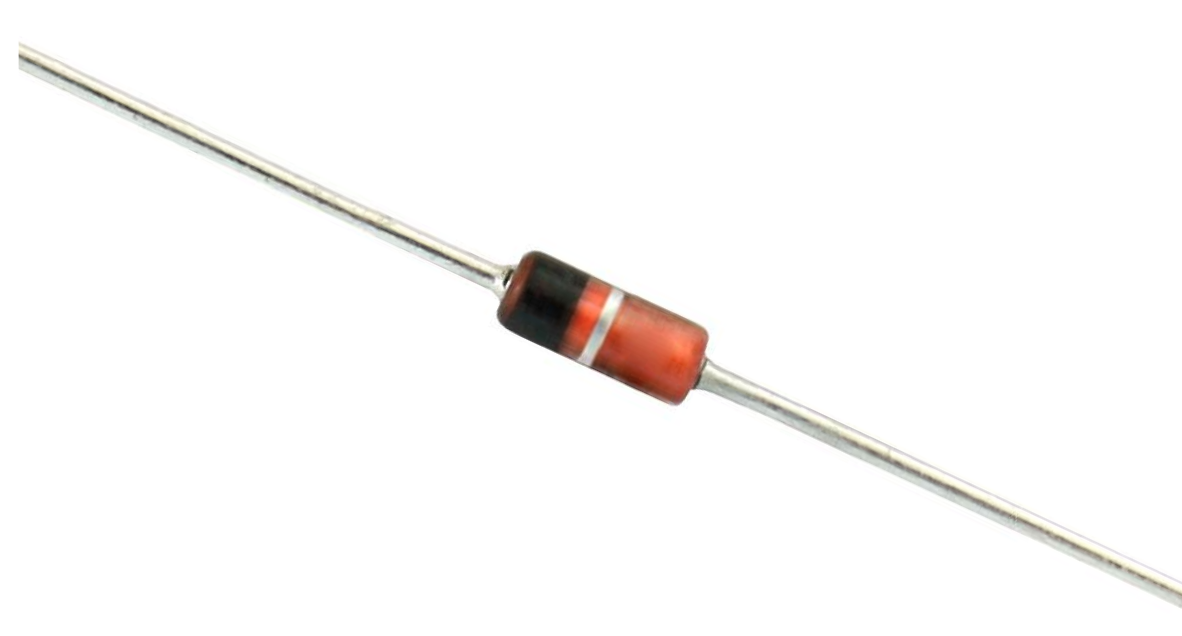
\includegraphics[width=.48\textwidth]{zener.png}}
\caption{Our zener diode}
\end{figure}

The zener diode was given proper voltages to work in reverse bias, specifically in the breakdown region. The overall circuit was identical to that of voltage regulator by zener diode. We gave particularly 5.0 V, 5.5V in two different runs from the powersource. The Zener diode regulated around 4.9 V. 

\begin{figure*}[hbt!]
\centering{\centering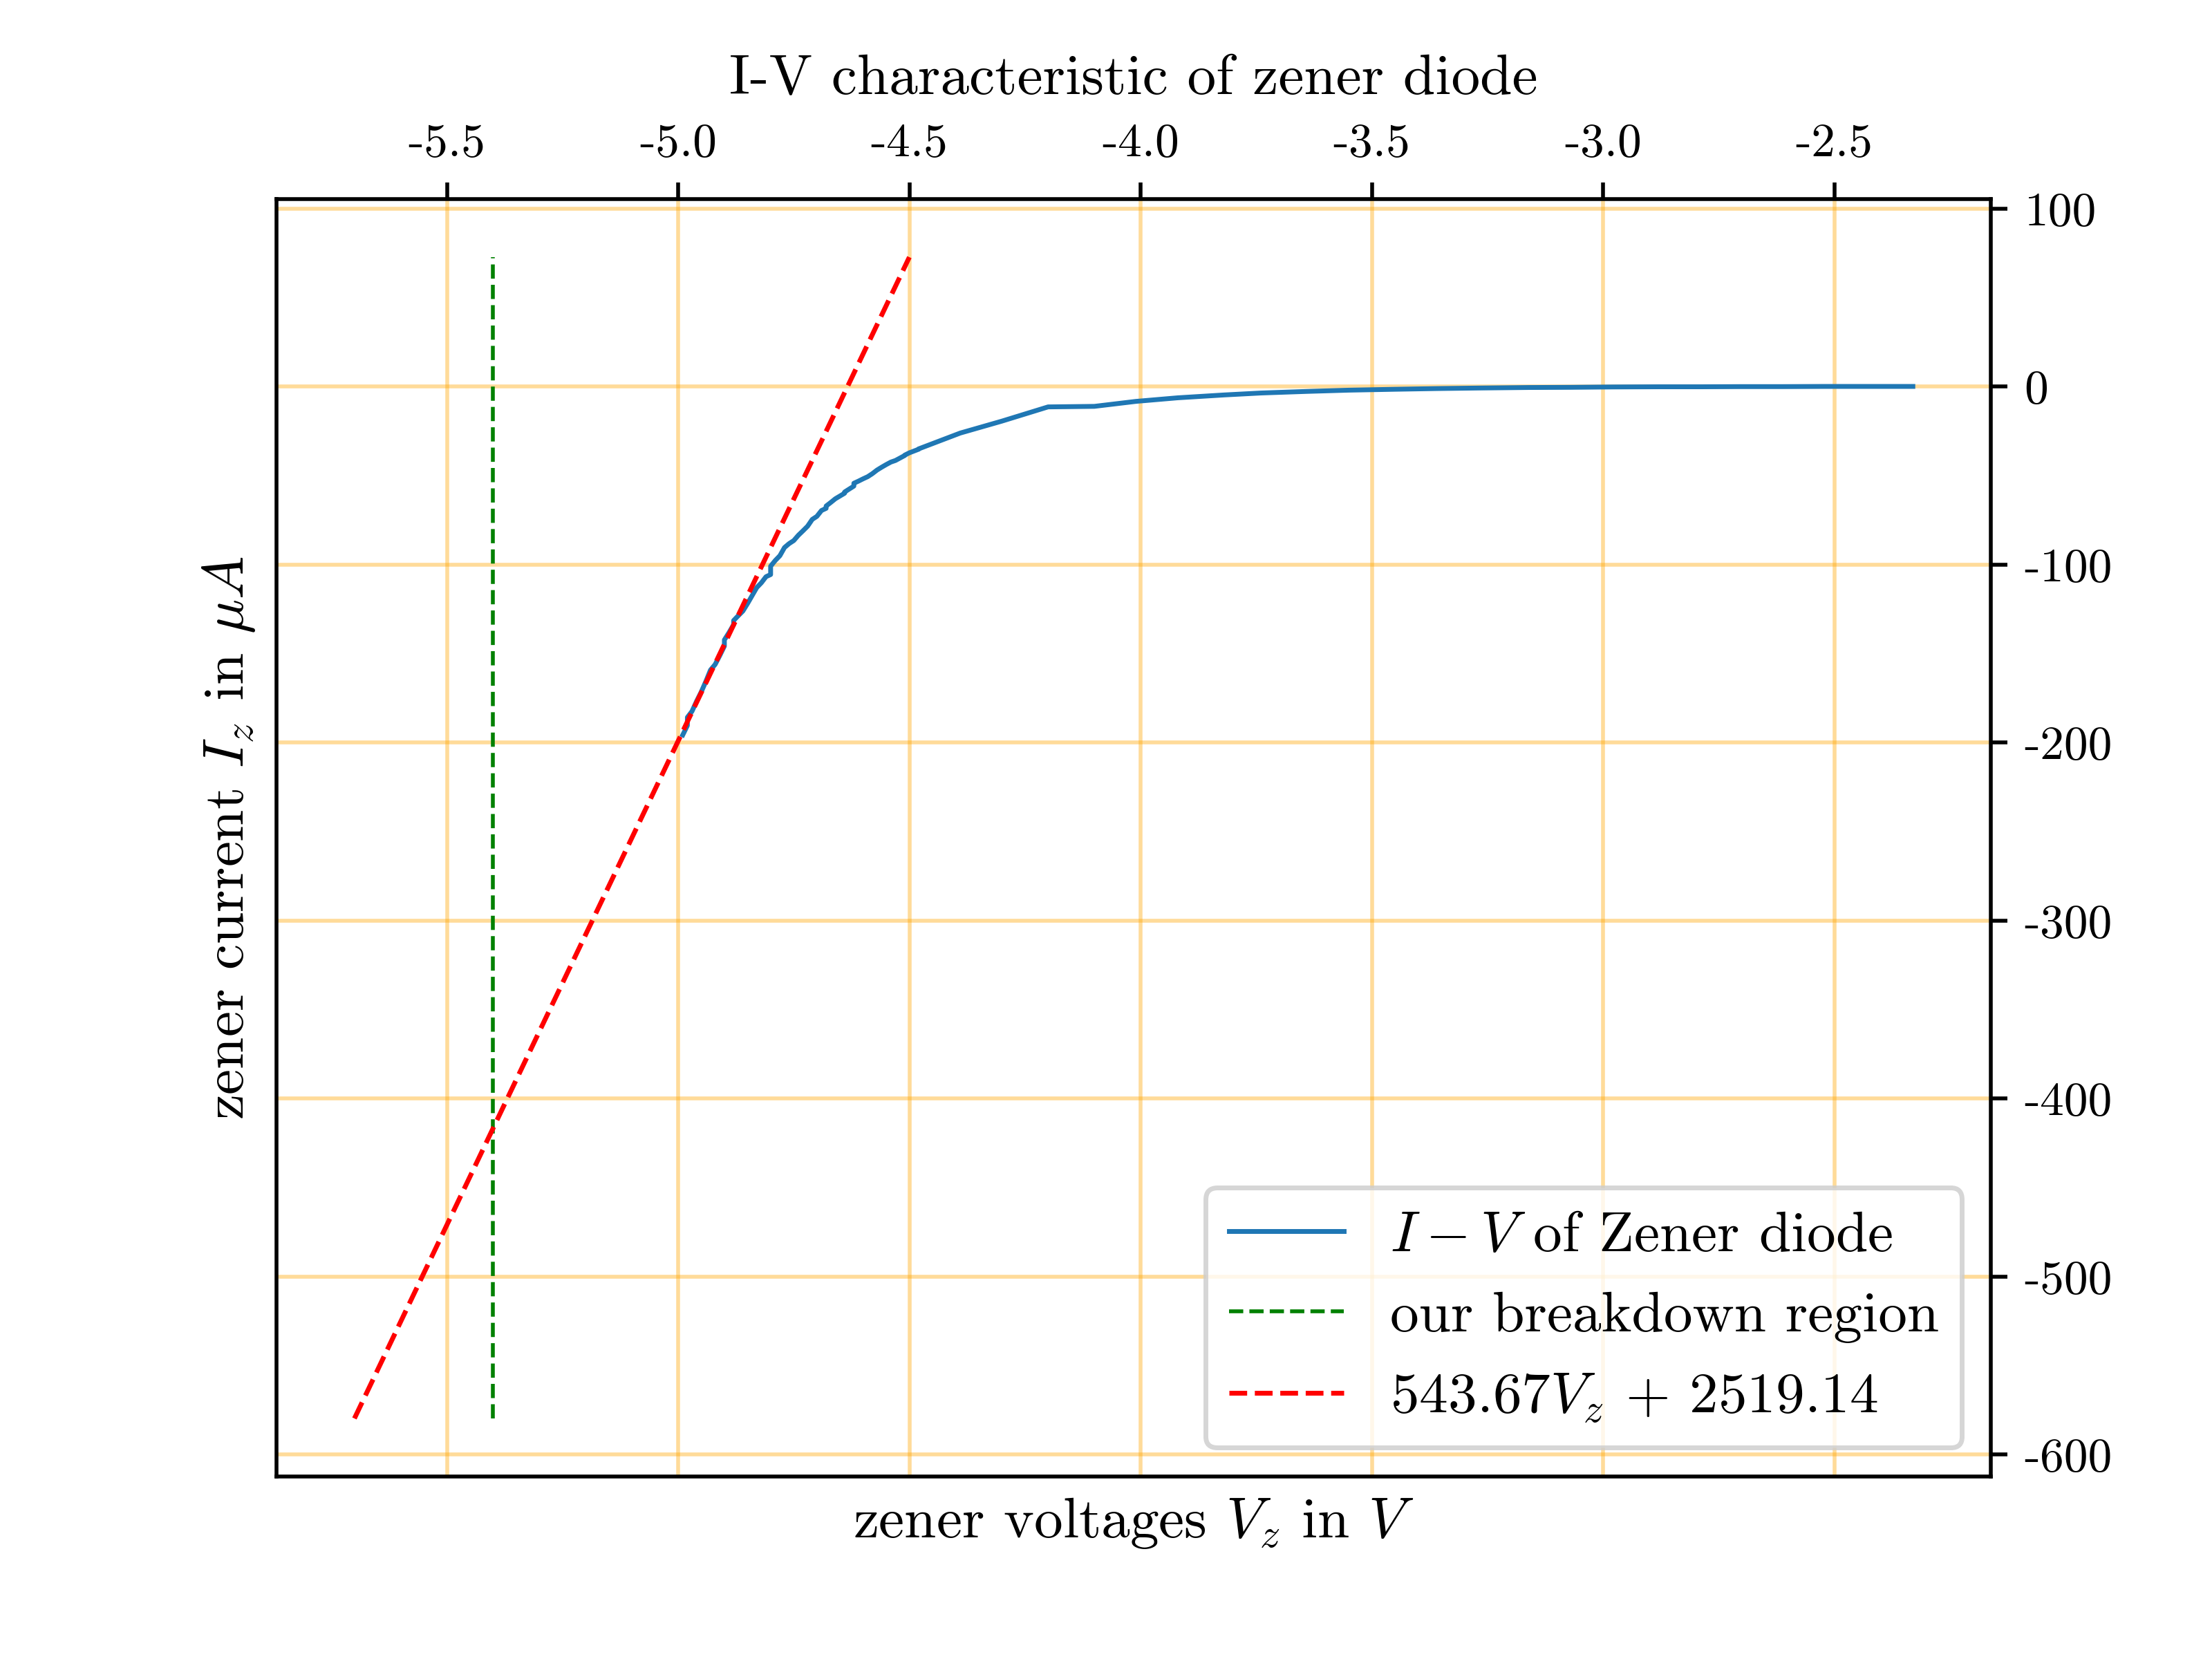
\includegraphics[width=1\textwidth]{zenerIV.png}}
\caption{current and voltage characterists of zener diode \label{exiv}}
\end{figure*}

Now, what we need is that fluctuation over the regulated DC voltage. These fluctuations have to be some function in the frequency domain as we assumed. This function must be made of different harmonics of sinusoidal waves with different phases and frequencies as thought by Fourier and his analysis. So basically we needed a system to measure different amplitudes of these harmonics at different frequencies to model our fluctuations. We needed a complete frequency spectrum at the particular bandwidth we are looking for in this analysis. The LOCK IN amplifier gives exactly that. 

\subsubsection{Theoritical noise spectral densities for our setup}

From equation \ref{theoryvn}, we can calculate total noise spectral density. we can get white noise spectral density via adding our thermal, shot, avalanche etc white noise source. 


\begin{itemize}

\item Shot noise and avalanche noise: From theoritical section we have equation \ref{thshots} and corrected with multiplicative factor $M$ aftre avalanche noise. Here, We have current values from current and voltage values from figure \ref{exiv}. At 5.4V it is $\approx -4.186 mA$. Also, $e = -1.602 \times 10^{-19} C$ and $M$ for silicon based zener diode is about 5 to 10,
\begin{align*}
  S(f) & = 2 (M+1) e I_0\\
  \\
  2(6)e|I_0| \geq & S(f) \geq 2(11)e|I_0|\\
  \\
  8.0371 \times 10^{-21} & V^2/Hz \geq  S(f) \geq \\
  1.4735 & \times 10^{-20} V^2/Hz\\
  \\
  0.8965 \times 10^{-10} &  V/\sqrt{Hz} \geq \sqrt{S(f)} \geq \\
  1.2139 & \times 10^{-10} V/\sqrt{Hz}
\end{align*}

\item Thermal noise: If we compute this values for our values, $K_B = 1.380649 × 10^{-23} m^2 kg s^{-2} K^{-1}$ and Trend from current and voltage relation is $0.00544V_z+0.02519$ gives impedence $R= 183.823 \Omega$

\begin{align}\label{thths}
  S(f) & = 4 K_B R\\
  S(f) & \approx 1.0147 \times 10^{-20} V^2/Hz \\
  \sqrt{S(f)} & \approx 1.0073 \times 10^{-10} V/\sqrt{Hz}
\end{align}


\end{itemize}



\subsection{Measuring instrument: LOCK IN amplifier}

LOCK IN amplifiers came in the 1930s and became very important in signal extraction from given frequency and phase. It is very helpful in measuring signals in a very noisy environment. It takes two inputs, one which is being measured and one which is given as a reference mono frequency signal. Reference signal gets multiplied with input signal and gives output through a process called Phase sensitive detection in which it uses homodyne detection scheme and filters out signal as DC component. We will see in a bit.\cite{srssr830}\cite{thinksrslockin}\cite{zhistpricipleoflockin}\cite{srssr830m}

\subsubsection{Phase sensitive detection}

In nutshell it uses frequency multiplication and generates double side bands which then pass through a low pass filter to extract signal. In figure \ref{fig:psd} you can see a signal first goes into a low noise differential amplifier which strengthens the signal. Signal Gets multiplied by another reference signal. This gives rise to two bands which pass through a low pass filter which cancels higher degree signal and only left is low frequency signal.


\begin{figure}[hbt!]
\centering{\centering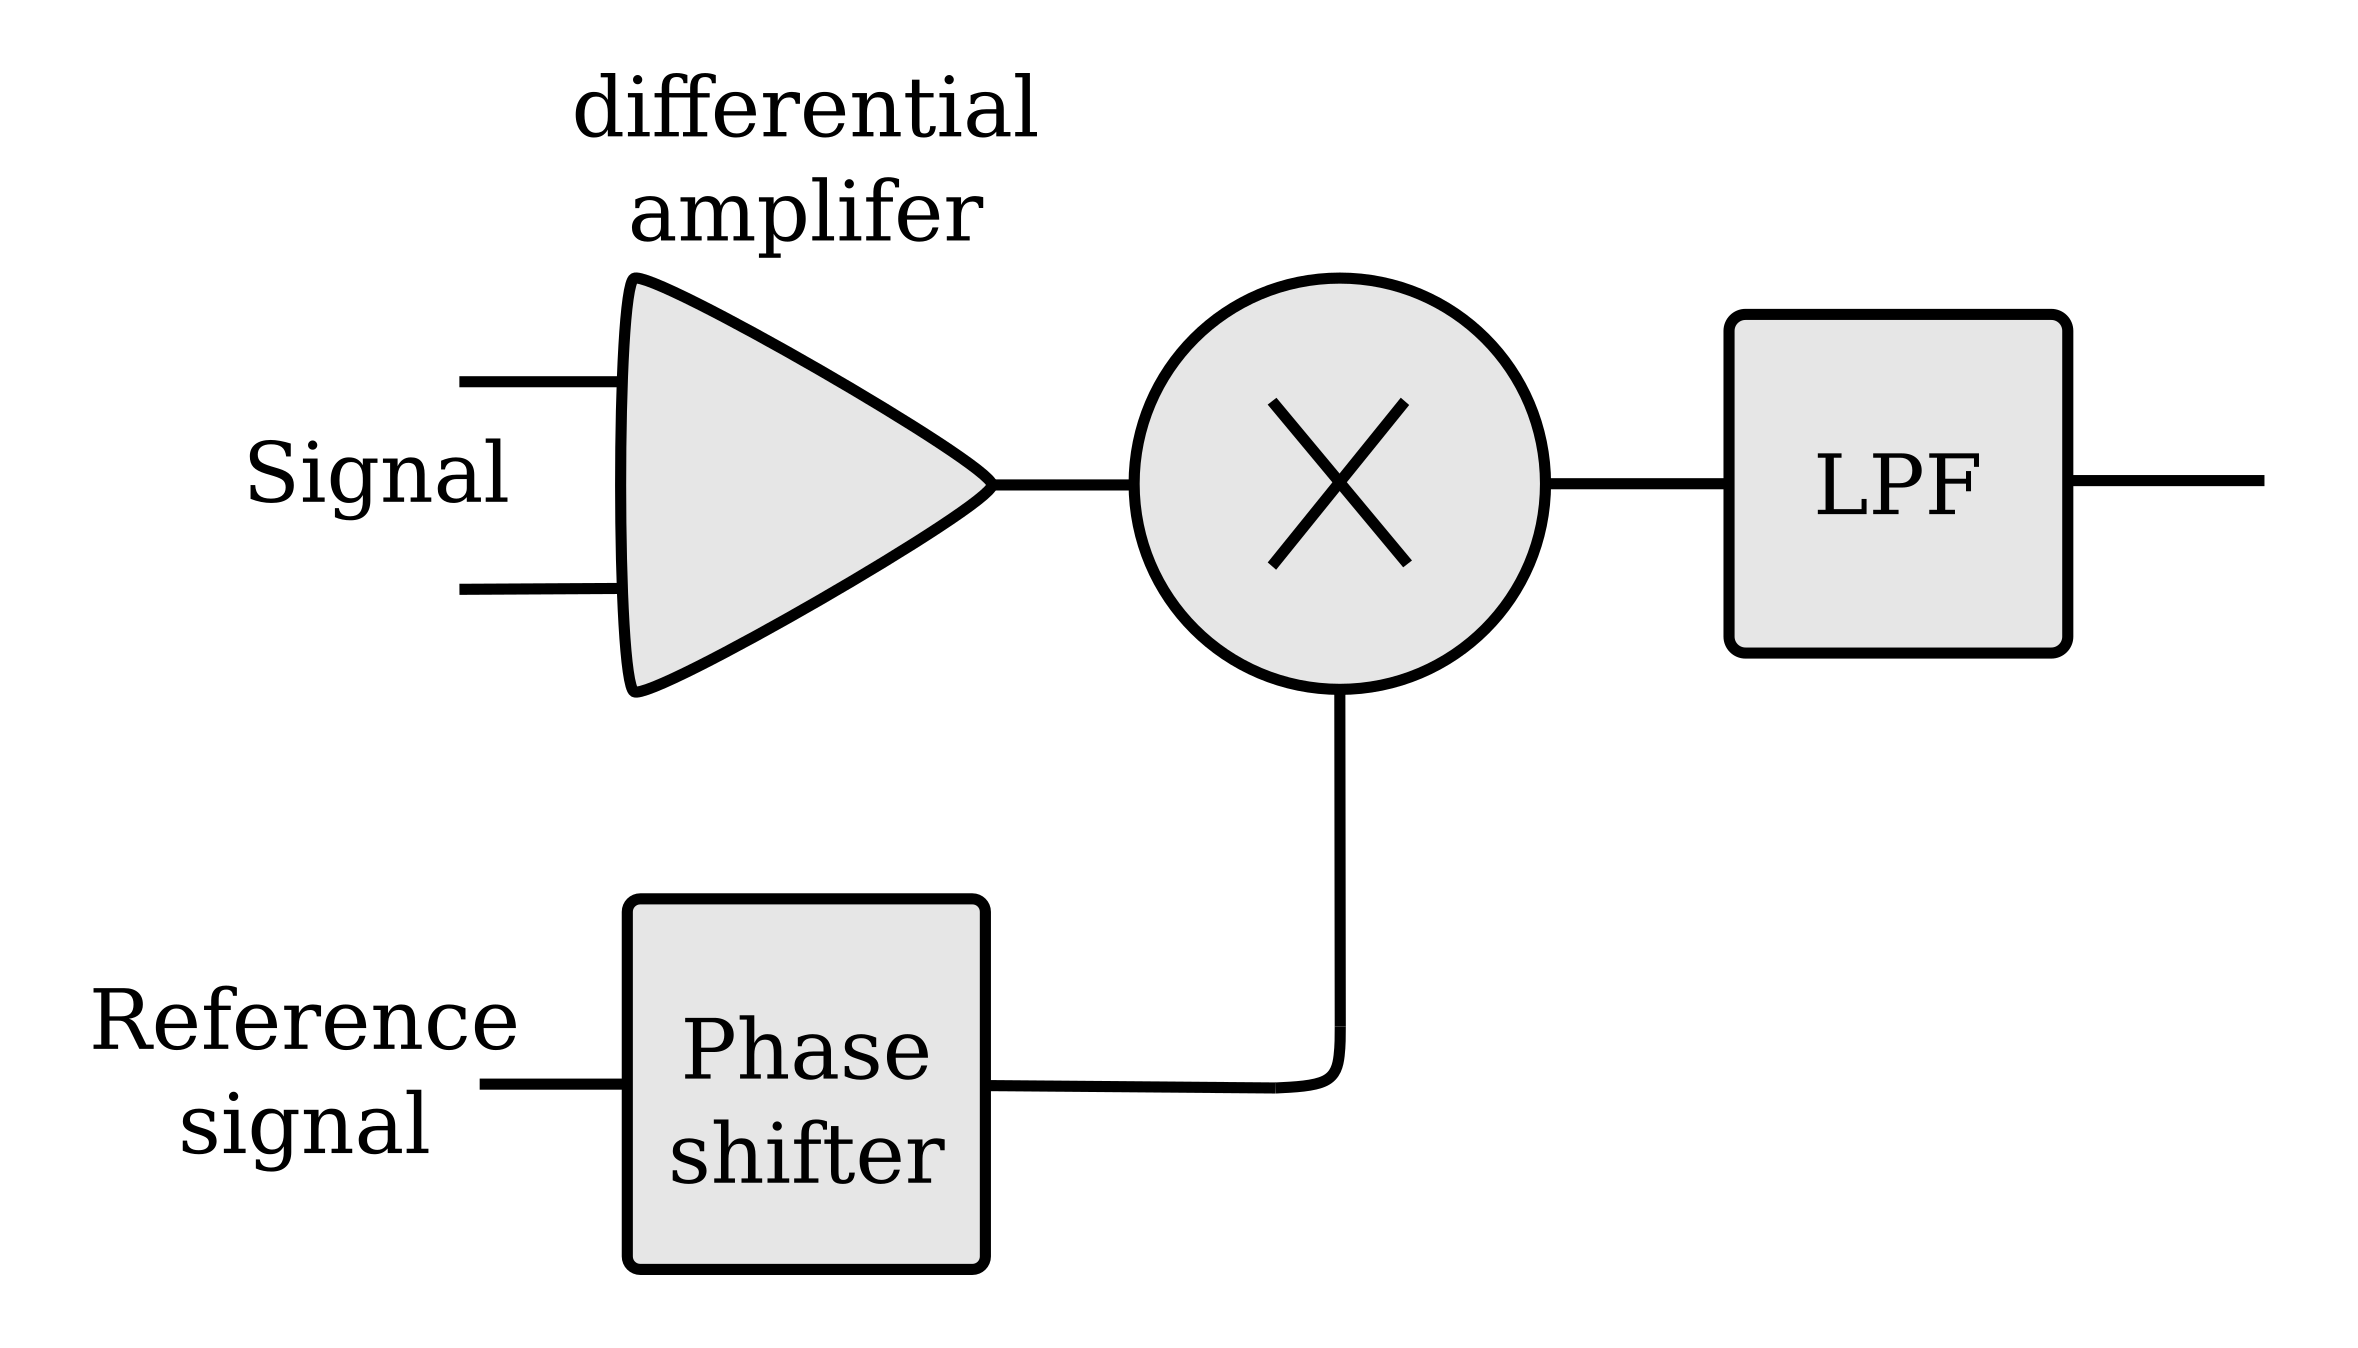
\includegraphics[width=.48\textwidth]{PSD.png}}
\caption{basic phase sensitive detector\label{fig:psd}}
\end{figure}

If we take signal $V_s(t)$ with frequency $w_s$, amplitude $A$ and phase $\theta$. 

\begin{align*}
V_{s}(t) & = A \cos(w_st+\theta)\\
\\
& = \frac{A}{2} (e^{i(w_st+\theta)}+e^{-i(w_st+\theta)})\\
\end{align*}

Reference signal can be taken as following,

\begin{align*}
V_r(t) & = B (e^{-i(w_rt+\phi)})
\end{align*}

In common settings, $\phi = 0$ and $B=1$,

\begin{align*}
V_r(t) & = e^{i(-w_rt)}
\end{align*}

Together after mixing the signals we have,

\begin{align*}
Z(t) & = V_s(t)\timesV_r(t)\\
\\
& = \frac{A}{2}(e^{i\left[ (w_s-w_r)t+\theta \right]}+e^{-i\left[ (w_s+w_r)t+\theta \right]})\\
\\
& = X(t)+Y(t)
\end{align*}

Making $w_s=w_r$ which makes subtraction vanishes and only one term with higher frequency lefts. Passing this signal through a low pass filter with very low cutoff gives only DC components and rejects noise even from neighbouring frequencies.


\begin{align*}
Z(t) & = \frac{A}{2}(e^{i \theta})
\end{align*}

Two component $X(t)$ and $Y(t)$ becomes,

\begin{align*}
X(t) & =\Re(Z(t))\\
\\
& =  \frac{A}{2}\cos(\theta)
\end{align*}

And,

\begin{align*}
Y(t) & = \Im(Z(t))\\
\\
& =  \frac{A}{2}\sin(\theta)
\end{align*}

So, Amplitude and Phase becomes, 

\begin{align*}
R & = \sqrt{X(t)^2+Y(t)^2}\\
\\
& =  \sqrt{(\frac{A}{2}\cos(\theta))^2+(\frac{A}{2}\sin(\theta))^2}\\
\\
& = \frac{A}{2}\\
\\
\Theta & = \arctan(\frac{Y}{X})
\end{align*}

So, the final product in PSD is the absolute amplitude of the signal and its phase. 

\subsubsection{Time Constant }

Time constant ($T$) is related to low pass filter in formal measurement system (PSD). most of the LOCK IN amplifier uses $n^{th}$ order buttersworth's filter as low pass filter.

so time constant value will be solely determined by R, C compoents of it.

\begin{align*}
T = 2 \pi R C
\end{align*}

\subsubsection{ENBW}

ENBW calculations and correction is very important in noise measurements. Same noise measurement in different settings is completely different in different settings and also different instruments. Before understanding how it affects measurement, the full form of it will be important ENBW: Equivalent Noise Bandwidth. This is determined by the cut off frequency of the low pass filter and  Roll off factor. The lock-in amplifier low pass filter is made of RC components ($n^{th}$ order buttersworth’s filter).  The roll of factor determined by order of low pass filter.  For Gaussian noise, the equivalent noise band-width (ENBW) of a low pass filter is the bandwidth of the perfect rectangular filter which passes the same amount of noise as the real filter.

This also determines measurement time delay. For example with 100ms time constant and 12dB/oct roll off it almost takes 0.7s to get its 99% value. This is shown in figure \ref{fig:ENBW}. 

\begin{figure}[hbt!]
  \centering\includegraphics[width=.48\textwidth,page=2,trim={9cm 13.8cm 2cm 8.5cm}, clip]{timeconstants_comparison.pdf}
\caption{This is how ENBW and response time related, here two LOCK in amplifier are given give ref}
  
\end{figure}


For SR830, this time constant and ENBW relation is given by the following table. 
\begin{center}
\begin{tabular}{| c | c | c |}
\hline
Slope & ENBW & Wait Time\\
\hline
6 dB/oct & $1/4T$ & $5T$ \\
12 dB/oct & $1/8T$ & $7T$ \\
18 dB/oct & $3/32T$ & $9T$ \\
24 dB/oct & $5/64T$ & $10T$\\
\hline
\end{tabular}
\end{center}
Here, T is time constant which is known. Output of LOCK IN amplifier is must be corrected by this values of ENBW for approximately true value of measurement.

\subsubsection{How LOCK IN amplifier measure noise}

LOCK IN amplifier can measure both amplitude and phase. As we have see from Phase Sensitive detection topic, It measures  $R$ as amplitude, but typical measurement also measure its $X$ and $Y$ components. So, $R^2=X^2+Y^2$, this give absolute amplitude. LOCK IN do time averaging to this measurement which is final $R$. The problem with only $R$ is that it does not give any information about its mean (typically mean is zero for noise measurement but offcet is probable). We assume in our measurement that there is zero offcet from mean, which means zero mean. \cite{zhistnoise}


Suppose noise power is following,

\begin{align*}
  P_w(t) & = n^2_w(t)\\
  P_w & = \frac{1}{T}\int_{T}P_w(t)dt\\
  P_w & = R^2 = X^2+Y^2
\end{align*}

We have ensebled average values after doing multiple value mean. So, final power density

\begin{align*}
  P_n & = \mathbb{E}({P_w})\\
  S_n & = \frac{P_n}{2\times ENBW}\\
  S_n & = \frac{\mathbb{E}(R^2)}{2 \times ENBW}
\end{align*}


Here, $S_n$ is Power spectral density measured in $V^2/Hz$. Spectral density is just $\sqrt{S_n}$ and measured in $V/\sqrt{Hz}$.

\subsubsection{LOCK IN amplifier over traditional measuring device/system}

For noise analysis LOCK IN amplifiers are the optimal choice. Traditional approaches deal with the first measurement of a small signal in the time domain. This signal gets amplified with additional noise from the amplifier. Also, amplifiers attenuates signals with its limited bandwidth which is a measure of concern for certain use case scenarios. This attenuated signal gets into some detector. For signal analysis, this signal must go into other  processes like analog to digital conversion then Fourier transformation. This whole process gives too much concerned noise which is not related to devices being analysed in our case the voltage regulator circuit. Alternative approach is to go with a LOCK IN amplifier. Which cancels out most burdens of traditional measurement steps. This whole combined help in reducing internal noise and increasing S/N ratio.
\\
\\
\emph{\large Pros of LOCK IN amplifier:}
\begin{itemize}
\item LOCK In amplifiers reduces attenuation of signal with increasing frequency since it does not measure signal in the whole frequency spectrum.
\item Increase S/N ratio over traditional amplifier circuit
\item Gives direct data into frequency domain
\end{itemize}\\
\\
\emph {\large Cons of LOCK IN amplifier:}
\begin{itemize}
\item Relatively expensive
\item Does not give information in time domain
\item Relatively slow for whole analysis of frequency domain (low but accurate resolution of frequency domain)
\end{itemize}

\subsection{SR830}

We used a LOCK IN amplifier from Stanford Research Systems. It is used to detect low amplitude signals as low as $10 nV/Hz$ and frequency as low as $1 mHz$.  and measure very small AC signals - upto few nanovolts. Accurate measurements may be made even when the small signal is obscured by noise sources many thousands of times larger.


Internal block diagram of SR830,

\begin{figure*}[hbt!]
  \centering\includegraphics[width=.8\textwidth,page=33,trim={2cm 4cm 1cm 7cm}, clip]{sr830m.pdf}
  \caption{Internal Block diagram of SR830}
\end{figure*}

\subsubsection{Inputs}
The LOCK IN amplifier takes two inputs, one for the main signal and another for reference signal. SR830 has an internal oscillator for reference signal (1 mHz to 102 kHz), this means that only one input is needed to be given. SR830 also takes external reference signals up to (up to 300 kHz), which can be useful for slightly higher frequencies. 

It can sense inputs from $2 nV$ to as high as 1V. The current input on the SR830 uses the A input BNC. The current input has a 1 kΩ input impedance and a current gain of either $10^6$ or $10^8$ Volts/Amp. Currents from 1 µA down to 2 fA full scale can be measured.

for more informations go to manual of SR830.\cite{srssr830m}

\subsubsection{Outputs}

SR830 can give outputs from range $\pm 10 V$ full scale and 10mA max current. the output can be showed to either both displays or can be output via BNC cables or can be logged out via interface.


\subsubsection{Interfacing}

The SR830 DSP Lock-in Amplifier may be remotely programmed via either the RS232 or GPIB (IEEE-488) interfaces. Any computer supporting one of these interfaces may be used to program the SR830. Both interfaces are receiving at all times, however, the SR830 will send responses to only one interface. Specify the output interface with the [Setup] key or use the OUTX command at the beginning of every program to direct the responses to the correct interface. The SR830 supports the IEEE-488.1 (1978) interface standard. It also supports the required common commands of the IEEE-488.2 (1987) standard. Before attempting to communicate with the SR830 over the GPIB interface, the SR830's device address must be set. The address is set with the [Setup] key and may be set between 1 and 30. The SR830 supports the IEEE-488.1 (1978) interface standard. It also supports the required common commands of the IEEE-488.2 (1987) standard. Before attempting to communicate with the SR830 over the GPIB interface, the SR830's device address must be set. The address is set with the [Setup] key and may be set between 1 and 30. The SR830 is configured as a DCE ( transmit on pin 3, receive on pin 2) device and supports CTS/
DTR hardware handshaking. The CTS signal (pin 5) is an output indicating that the SR830 is ready, while the DTR signal (pin 20) is an input that is used to control the SR830's data transmission. If desired, the handshake pins may be ignored and a simple 3 wire interface (pins 2,3 and 7) may be used. The RS232 interface baud rate and parity must be set. These are set with the [Setup] key. The RS232 word length is always 8 bits. To assist in programming, the SR830 has 4 interface status indicators. The ACTIVE indicator flashes whenever a character is received or transmitted over either interface. The ERROR indicator flashes when an error, such as an illegal command, or parameter out of range, has been detected. The REMOTE indicator is on whenever the SR830 is in a remote state (front panel locked out). The SRQ indicator is on when the SR830 generates a service request. SRQ stays on until a serial poll is completed. Communications with the SR830 uses ASCII characters. Commands may be in either UPPER or lower case and may contain any number of embedded space characters. A command to the SR830 consists of a four character command mnemonic, arguments if necessary, and a command terminator. The terminator must be a linefeed <lf> or carriage return <cr> on RS232, or a linefeed <lf> or EOI on GPIB.


Example of commands,

\begin{tabular}{p{0.26\linewidth} p{0.48\linewidth}}
 FREQ 10E3 <lf> & Set the internal reference frequency to 10000 Hz (10 kHz)\\
 *IDN? <lf> & Queries the device identification  
\end{tabular}
